\documentclass[tikz,border=10pt]{standalone}
% Scale: s = 0.012739 cm/px (STYLE METRICS), A at origin, y flipped
\begin{document}
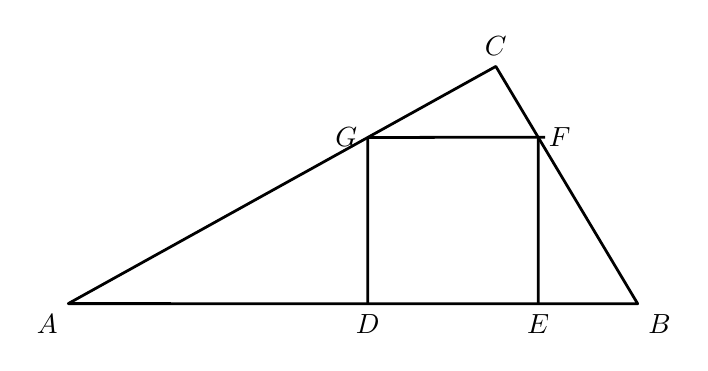
\begin{tikzpicture}[line width=1.0pt, line join=round]
  % Named coordinates (cm)
  \coordinate (A) at (-0.0003102351477517473,0.000834388321584667);
  \coordinate (B) at (7.23108880657408,-0.0003220442036357962);
  \coordinate (C) at (5.42975334920868,3.0133066084872464);
  \coordinate (D) at (3.8033588614209966,0.00022611229713853653);
  \coordinate (E) at (5.967037353512635,-0.00011989933427081212);
  \coordinate (F) at (5.967375418480566,2.113866548252326);
  \coordinate (G) at (3.803696445950794,2.1112082861796106);
  % Right end of horizontal segment (x=554 px at y=148 px), unchanged
  \coordinate (H2) at (6.056446457158239,2.1138526648459366);

  % Triangle ABC (solid black)
  \draw[black] (A) -- (B) -- (C) -- cycle;

  % Horizontal line from G (starts exactly at vertex G) to right end
  \draw[black] (G) -- (H2);

  % Vertical segments G-D and F-E
  \draw[black] (G) -- (D);
  \draw[black] (F) -- (E);

  % Labels in math mode with metrics font
  \node[below left, font=\fontsize{10}{12}\selectfont] at (A) {$A$};
  \node[below right, font=\fontsize{10}{12}\selectfont] at (B) {$B$};
  \node[above, font=\fontsize{10}{12}\selectfont] at (C) {$C$};
  \node[below, font=\fontsize{10}{12}\selectfont] at (D) {$D$};
  \node[below, font=\fontsize{10}{12}\selectfont] at (E) {$E$};
  \node[right, font=\fontsize{10}{12}\selectfont] at (F) {$F$};
  \node[left, font=\fontsize{10}{12}\selectfont] at (G) {$G$};
\end{tikzpicture}
\end{document}
% GEOAGENT_REPAIR_V1 c18a466396f54661 39ace92d0ac370baa6558a38fc117033e14f816d64a36073f426052862172c9e
